%!TEX root = ../dokumentation.tex

\chapter{Quiescence Search}\label{ch:quiescence}
Dieses Kapitel beschäftigt sich mit der konkreten Zielsetzung dieser Arbeit: Eine Ergänzung der Schach-KI, sodass die Quiescence Search implementiert ist und das Programm somit effektivere Züge berechnen kann. 

\section{Motivation}\label{section:motivation}
Zunächst gilt zu klären, welche Motivation beziehungsweise welche Problemstellung der Notwendigkeit der Quiescence Search zugrunde liegt. Die Bezeichnung für das Problem, welches bei der vorhandenen Implementierung des Algorithmus auftritt, lautet \textit{Horizonteffekt}. Aufgrund der Tatsache, dass der Algorithmus mit einer festen Tiefe arbeitet, existiert für das Programm ein metaphorischer Horizont, über welchen es nicht hinausschauen kann. \textit{Oxford Reference} definiert den Begriff "`Horizonteffekt"' folgendermaßen: "`\textit{The horizon effect refers to the fact that interesting results will always exist beyond any depth D and therefore in any given search will not be discovered} […]"'\footcite{oxford}.

Abbildung~\ref{fig:problem} zeigt eine beispielhafte Aufstellung der Figuren auf einem Schachbrett. Aufgabe der KI ist es nun, den bestmöglichen Zug zu finden\footnote{Um das Beispiel möglichst einfach zu halten, wird angenommen, dass die KI mit einer Tiefe von $1$ rechnet. Für die Erklärung der Problemstellung macht dies jedoch keinen Unterschied, da sich das Beispiel übertragen lässt}.  Das Programm wird schnell erkennen, dass die Dame auf B2 den Springer auf B7 schlagen kann. Da der Horizont an dieser Stelle "`endet"', schätzt das Programm eben diesen Zug als den besten ein und gibt ihn zurück. Wäre die Suchtiefe jedoch um eine Ebene tiefer gewesen, hätte das Programm diesen Zug ausgeschlossen, da, nachdem die Dame den Springer geschlagen hat, der Läufer auf A8 die Dame direkt schlagen kann. Da eine Dame jedoch deutlich mehr wert ist als ein Springer -- in der vorhandenen Implementierung ist eine Dame 9 Bauern wert, ein Springer jedoch nur 3,2 Bauern -- handelt es sich um einen sehr schlechten Zug.

\begin{figure}[H]
	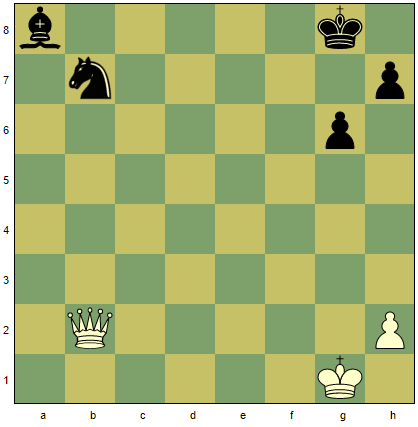
\includegraphics[width=.90\textwidth]{problem.png}
	\caption{Beispiel-Zustand für ein Schachbrett: Weiß kann im nächsten Zug einen Springer schlagen\footnotemark}
	\label{fig:problem}
\end{figure}
\footnotetext{\cite{nextchessmove}}

Ein weiteres Beispiel für den Horizonteffekt ist die scheinbare Vermeidung von schlechten Positionen: Das Programm erkennt eine schlechte Position, beispielsweise den Verlust einer Dame. Nun errechnet die KI einen Pfad, in dem diese Dame scheinbar nicht verloren wird; in der Realität hat das Programm den Verlust jedoch nur "`über"' den Horizont geschoben, sodass der Verlust der Dame unausweichlich ist -- zusätzlich hat das Verschieben des Problems womöglich eine insgesamt schlechtere Position hervorgerufen, als wenn die Dame direkt geopfert worden wäre.

Diese Beispiele verdeutlichen, dass, bei taktischen Zügen, eine tiefere Evaluation nicht nur sinnvoll sondern auch notwendig ist, um die Effektivität der Schach-KI zu steigern. Wird bei der tieferen Evaluation festgestellt, dass der Zug keine schlechtere Position hinter dem Horizont hervorruft, spricht man von einer \textit{ruhigen} Stellung, was auch die Bezeichnung der \textit{Ruhesuche} erklärt.

\section{Funktionsweise}
Bevor die Quiescence konkret implementiert werden kann, muss geklärt werden, wie sie funktioniert und wann sie eingesetzt wird.

In Abschnitt~\ref{section:motivation} wurden \textit{taktische Züge} erwähnt. Das \textit{Chess Programming Wiki} definiert den Begriff folgendermaßen: "`\textit{Tactical moves in the context of chess program move classification are moves which immediate change material balance and capture a piece or cause a promotion} […]"'\footcite{chessprogramming}. Es handelt sich also bei taktischen Züge um das Schlagen von Figuren respektive um das Aufwerten eines Bauern. Die Erweiterung des Algorithmus muss also dann eine tiefere Suche durchführen, wenn ein solcher taktischer Zug der zuletzt analysierte war. 

Die Position in der Implementierung, an der die Quiescence Search eingesetzt werden muss, lässt sich ebenfalls definieren: So muss die Funktion für die Quiescence Search dann aufgerufen werden, wenn das Programm an der Suchtiefe angekommen ist. Innerhalb der Funktion wird dann geprüft, ob der letzte Zug ein taktischer Zug war, um eventuell tiefer zu suchen. Die tiefere Suche wird lediglich durch einen erneuten Aufruf der Minimax-Funktion umgesetzt.

\section{Implementierung}
Dieser Abschnitt zeigt die Implementierung der Quiescence Search. Außerdem wird erläutert, wie die korrekte Funktionsweise der Quiescence Search geprüft wurde.

\begin{lstlisting}[caption=Erweiterung der Funktion des Minimax-Algorithmus für die Verwendung von Quiescence Search, label=lst:erweiterung]
	@memoize_minimax
	def minimax(board, depth, alpha, beta, is_quiesce):
		# ...
		if depth == 0 or not board.legal_moves:
			value = static_eval(board, is_endgame(board))
			if is_quiesce:
				return value
			return quiesce(board,alpha,beta,value)
		# ...
\end{lstlisting}

Der Code-Ausschnitt~\ref{lst:erweiterung} zeigt den Teil der Minimax-Funktion, der für die Verwendung der Quiescence Search erweitert wurde. Zum einen wurde der Funktion der Parameter \texttt{is\_quiesce} hinzugefügt (dieser wird bei der Erläuterung der Funktion \texttt{quiesce} genauer erklärt), zum anderen wurde der Aufruf der Funktion \texttt{quiesce} mit den Parametern \texttt{board}, \texttt{alpha}, \texttt{beta} und \texttt{value}. Der Parameter \texttt{board} stellt dabei den aktuellen Spiel-Zustand dar, die Werte \texttt{alpha} und \texttt{beta} sind die Schranken des Alpha-Beta-Prunings. Diese drei Werte werden schlicht übernommen, da die Minimax-Funktion ebenfalls mit diesen Parametern aufgerufen wird. Der letzte Parameter \texttt{value} hingegen ist der Rückgabewert der Evaluierungsfunktion \texttt{static\_eval}.

Bevor die eigentliche Quiescence-Search-Funktion \texttt{quiesce} vorgestellt wird, wird in dem Code-Ausschnitt~\ref{lst:pieces} die Hilfsfunktion \texttt{get\_pieces\_sum} gezeigt. Diese Funktion hat als Eingabeparameter \texttt{board}, den aktuellen Spielzustand, und berechnet lediglich die Figurenanzahl -- beziehungsweise die Werte, sodass also eine Dame den Rückgabewert stärker erhöht als ein Bauer -- der beiden Spieler. Diese Funktion ist notwendig, um zu überprüfen, ob ein Zug ein taktischer Zug war, also eine Veränderung der Figurenanzahl/-werte verursacht hat.

\begin{lstlisting}[caption=Hilfsfunktion für die Differenzierung taktischer Züge, label=lst:pieces]
	def get_pieces_sum(board):
    	value = 0
    	for piece_type in range(1,6):
        	value += len(board.pieces(piece_type,chess.WHITE))
        	value += len(board.pieces(piece_type,chess.BLACK))
    	return value
\end{lstlisting}

Es existieren zudem zwei Konstanten, \texttt{ENABLE\_QUIESCENCE\_SEARCH} und \texttt{QUIESCE\_DEPTH}. Bei der ersten Konstante handelt es sich um ein \textit{Flag}, um die Ruhesuche zu deaktivieren. Dies ist für den Test der Funktion notwendig, da überprüft wird, ob das Programm mit Quiescence Search einen besseren Zug spielt, als ohne. Die Konstante \texttt{QUIESCE\_DEPTH} steht standardmäßig auf $2$ und legt fest, wie tief das Programm in der Ruhesuche weiterhin sucht. Eine solche Begrenzung ist notwendig, da das Programm andernfalls womöglich sehr viele Ebenen tiefer rechnen würde, wenn in mehreren aufeinanderfolgenden Zügen eine Figur geschlagen oder aufgewertet werden kann. In einer ersten Implementierung existierte diese Begrenzung nicht, was einen Rekursions-Fehler zur Folge hatte, da das Programm letztlich zu tief analysiert hatte.

\begin{lstlisting}[caption=Funktion für die Implementierung der Ruhesuche, label=lst:quiesce]
	def quiesce(board,alpha,beta,value):
    	if not ENABLE_QUIESCENCE_SEARCH:
			return value
		pieces_after_move = get_pieces_sum(board)
		move = board.pop()
		pieces_before_move = get_pieces_sum(board)
		board.push(move)
		if(pieces_after_move != pieces_before_move):
			value = minimax(board,QUIESCE_DEPTH,max(value,alpha),beta,True)
		return value
\end{lstlisting}

Der Code-Ausschnitt~\ref{lst:quiesce} zeigt nun die komplette Funktion \texttt{quiesce}, welche die Ruhesuche implementiert. Hierfür wird zunächst der bereits evaluierte Wert \texttt{value} zurückgegeben, falls die Quiescence Search deaktiviert ist (erkennbar durch das Flag \texttt{ENABLE\_QUIESCENCE\_SEARCH}). Andernfalls wird zunächst die Summe der Figurenwerte aktuell -- also nach dem letzten evaluierten Zug --, danach die Summe der Figurenwerte vor jenem letzten Zug verglichen. Stimmen diese beiden Werte nicht überein, so besteht hier die beschrieben Notwendigkeit, die Quiescence Search anzuwenden. In diesem Fall wird die Minimax-Funktion mit den folgenden Parametern aufgerufen:

\begin{itemize}
	\item \texttt{board}: Hier wird der aktuelle Spielzustand \texttt{board} übernommen, der der Funktion \texttt{quiesce} übergeben wurde. Der Spielzustand ist nicht verändert, da der \texttt{move}, welcher zuerst rückgängig gemacht wurde (um die Anzahl/Werte der Figuren zu erfassen), wieder "`gespielt'" wurde
	\item \texttt{depth}: Hier wird die Konstante \texttt{QUIESCE\_DEPTH}, welche oben erwähnt wurde, übergeben. Es wird somit festgelegt, wie weit die Ruhesuche tiefer sucht, falls ein taktischer Zug der letzte analysierte Zug war
	\item \texttt{alpha}: Hier wird der größere Wert von \texttt{value} und \texttt{alpha} übergeben
	\item \texttt{beta}: Hier wird lediglich der Wert der Variable \texttt{beta} übernommen, welcher bei Aufruf der Funktion übergeben wurde
	\item \texttt{is\_quiesce}: Hier wird der Wert \texttt{True} übergeben. Dadurch wird erreicht, dass, bei der Suchtiefe $0$, nicht erneut die Quiescence-Search-Funktion aufgerufen wird. In einer ersten Implementierung führte dies zu einem Rekursionsfehler
\end{itemize}

\section{Testen der Programm-Erweiterung}
Um zu überprüfen, ob die Erweiterung, welche die Quiescence Search implementiert, wie erwartet funktioniert, wurde ein weiterer Test geschrieben. Zu diesem Zweck wurde das Szenario aus Abbildung~\ref{fig:problem} übernommen: Das Programm wurde zunächst normal aufgerufen, sodass die Erweiterung für die Quiescence Search in Kraft tritt. Aus Gründen der Einfachheit, wird die Minimax-Funktion mit einer Tiefe von $1$ aufgerufen. Der Code-Ausschnitt~\ref{lst:testone} zeigt dies.

\begin{lstlisting}[caption=Test für die Quiescence Search (normaler Aufruf), label=lst:testone]
	%%time
	CACHE = {} # Has to be cleared for this test to work
	board,move = perform_move(chess.Board("b3k3/1n5p/6p1/8/8/8/7P/1Q4K1 w - - 0 1"),1, True)
	assert str(move) != "b1b7"
\end{lstlisting}

Der Cache -- welcher für die \textit{Memoization} verwendet wird -- muss geleert werden, da das Ergebenis sonst verfälscht werden könnte. Außerdem wird die Funktion \texttt{perform\_move} verwendet, welche jedoch lediglich das mehrfache Schreiben gleicher Anweisungen verhindert. Anschließend wird geprüft, ob es sich bei dem errechneten Zug \textbf{nicht} um den Zug \textit{b1b7}, also die Dame auf B7, wo sie im nächsten Zug geschlagen werden kann, handelt. Abbildung~\ref{fig:testone} zeigt, dass dies der Fall ist und die Ruhesuchenerweiterung somit eingreift und auch den taktischen Zug erkannt hat.

\begin{figure}[H]
	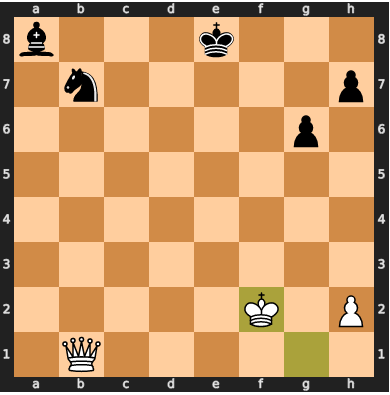
\includegraphics[width=.90\textwidth]{testone.png}
	\caption{Korrekte Anwendung der Quiescence Search: Der scheinbar gute Zug wird nicht gewählt, obwohl die Minimax-Tiefe auf $1$ gesetzt ist}
	\label{fig:testone}
\end{figure}

Zur Kontrolle des Tests wird der Test erneut aufgerufen, jedoch wird bei dem zweiten Mal das Flag \texttt{ENABLE\_QUIESCENCE\_SEARCH} auf \texttt{False} gesetzt, sodass die Erweiterung der Ruhesuche nicht verwendet wird (Der Code-Ausschnitt~\ref{lst:erweiterung} zeigt dies). Der Code-Ausschnitt~\ref{lst:testtwo} zeigt der Vollständigkeit halber auch den Code für diesen zweiten Test.

\begin{lstlisting}[caption=Test für die Quiescence Search (Aufruf mit deaktivierter Ruhesuche), label=lst:testtwo]
	%%time
	ENABLE_QUIESCENCE_SEARCH = False
	CACHE = {} # Has to be cleared for this test to work
	board,move = perform_move(chess.Board("b3k3/1n5p/6p1/8/8/8/7P/1Q4K1 w - - 0 1"),1, True)
	assert str(move) == "b1b7"
	ENABLE_QUIESCENCE_SEARCH = True
\end{lstlisting}

Es ist zu sehen, dass der Test nahezu gleich ist, jedoch einen anderen errechneten Zug erwarten, nämlich den scheinbar guten Zug \textit{b1b7}. Abbildung~\ref{fig:testtwo} zeigt, dass das Ergebnis dieses Tests auch das eben erwartete ist: Das Programm denkt, aufgrund der Suchtiefe, dass es den besten Zug gefunden hat; der Horizonteffekt tritt ein.

\begin{figure}[H]
	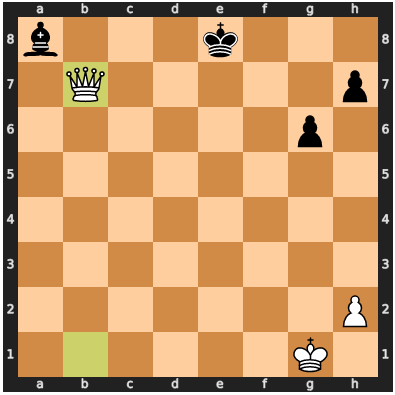
\includegraphics[width=.90\textwidth]{testtwo.png}
	\caption{Kontrolltest: Ohne Quiescence Search wählt das Programm einen schlechten Zug, welchen es allerdings aufgrund des Horizonteffekts nicht als solchen erkennt}
	\label{fig:testtwo}
\end{figure}

\section{Performanz-Analyse}
Letztlich gilt es zu untersuchen, inwiefern die Verbesserung der Zugberechnung Auswirkungen auf die Performanz und Berechnungsdauer des Programms hat. Hierfür wurden zwei Ansätze -- bei beiden Ansätzen wird das Programm einmal ohne Quiescence Search und einmal mit Quiescence Search aufgerufen -- analysiert:

\begin{enumerate}
	\item gleiche Tiefe bei beiden Aufrufen
	\item Tiefe beim Aufruf mit Quiescence Search ist um $1$ verringert, dafür hat die erweiterte Suche eine Tiefe von $1$
\end{enumerate}

Bei der zweiten Variante handelt es sich also de facto um keine tiefere Suche als bei dem Vergleichswert ohne Quiescence Search; stattdessen wird generell weniger tief gesucht und nur bei taktischen Zügen eine tiefere Suche vorgenommen. Wenn ein starker Fokus auf die Berechnungsdauer des Programms gelegt wird, wäre die zweite Variante als Ansatz denkbar.

HIER DANN ERGEBNISSE EINFÜGEN